\chapter{Domain and Segment Setup} \label{chap:domainsetup}

This chapter explains how a {\ViennaGrid} domain can be filled with cells. Since this
is a necessary step in order to do anything useful with {\ViennaGrid}, it is explained in detail in the following.
Existing file readers and writers are explained in Chapter \ref{chap:io}.

\TIP{A tutorial code can be found in \texttt{examples/tutorial/domain\_setup.cpp}.}

In the following, the simple triangular mesh shown in Fig.~\ref{fig:sampledomain} will be set up.
Thus, the domain type using the provided configuration class for two-dimensional triangular classes will be used:
\begin{lstlisting}
 typedef viennagrid::config::triangular_2d                      ConfigType;
 typedef viennagrid::result_of::domain<ConfigType>::type        DomainType;
 typedef viennagrid::result_of::segmentation<DomainType>::type  SegmentationType;
 typedef viennagrid::result_of::segment<SegmentationType>::type  SegmentType;

 // The domain to be set up in the following
 DomainType domain;
 
 // The segmentation for the example mesh in Figure 4.1
 SegmentationType segmentation(domain);
 
 // Segment 0, the left one
 SegmentType segment_0 = segmentation.make_segment();
 // Segment 1, the right one
 SegmentType segment_1 = segmentation.make_segment();
\end{lstlisting}
If these lines are used inside a template class or template function, an additional \lstinline|typename| needs to be put after \lstinline|typedef| in the second line.
The created domain object will be filled with vertices and cells in the following.

\begin{figure}[tb]
\centering
 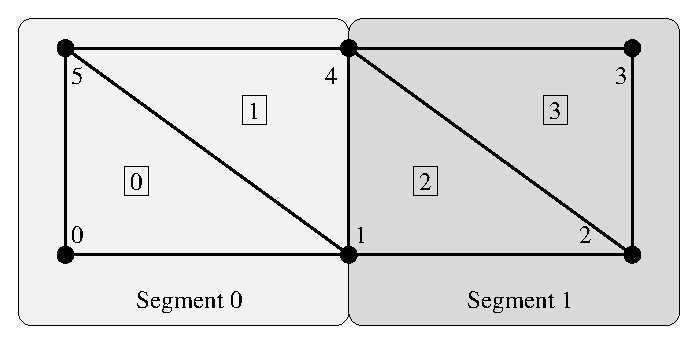
\includegraphics[width=0.65\textwidth]{figures/sampledomain.eps}
 \caption{An exemplary mesh for demonstrating the use of {\ViennaGrid}. Cell-indices are boxed.}
 \label{fig:sampledomain}
\end{figure}

\pagebreak

\section{Adding Vertices to a Domain or Segment}
Since vertices carry geometric information by means of an associated point type, we first obtain the respective point type from the meta-function \lstinline|point<>|:
\begin{lstlisting}
 typedef viennagrid::result_of::point<DomainType>::type    PointType;
\end{lstlisting}
This already allows us to add the vertices shown in Fig.~\ref{fig:sampledomain} one after another to the domain by using \lstinline|make_vertex|. This function returns a handle to the created vertex. We might need this handle so we have to define a type for our vertex handle:
\begin{lstlisting}
 typedef viennagrid::result_of::handle<
      DomainType,
      viennagrid::vertex_tag
  >::type    VertexHandleType;
\end{lstlisting}
Much simpler is the use of the convenience meta function \lstinline|vertex_handle|
\begin{lstlisting}
 typedef viennagrid::result_of::vertex_handle<
      DomainType
  >::type    VertexHandleType;
\end{lstlisting}
One example to add the first vertex is to push the respective point to the domain:
\begin{lstlisting}
 PointType p(0,0);
 // add vertex #0
 VertexHandleType vh0 = viennagrid::make_vertex(domain, p);
\end{lstlisting}
The member function \lstinline|make_vertex| adds the vertex to the domain and assigns an ID.

To push the next vertex, one can either reuse the existing vertex:
\begin{lstlisting}
 p[0] = 1.0;
 p[1] = 0.0;
 // add vertex #1
 VertexHandleType vh1 = viennagrid::make_vertex(domain, p);
\end{lstlisting}

\pagebreak

or directly construct the respective points in-place:
\begin{lstlisting}
 // add vertex #2
 VertexHandleType vh2 = viennagrid::make_vertex(domain, PointType(2,0));
 // add vertex #3
 VertexHandleType vh3 = viennagrid::make_vertex(domain, PointType(2,1));
 // add vertex #4
 VertexHandleType vh4 = viennagrid::make_vertex(domain, PointType(1,1));
 // add vertex #5
 VertexHandleType vh5 = viennagrid::make_vertex(domain, PointType(0,1));
\end{lstlisting}

It is also possible to explicitly specify the ID for a new vertex:
\begin{lstlisting}
 typedef viennagrid::result_of::vertex<DomainType>::type   VertexType;
 typedef viennagrid::result_of::id<VertexType>::Type       VertexIDType;
 
 VertexHandleType some_vh = viennagrid::make_vertex(domain, VertexIDType(42), PointType(0,0));  // add some vertex with ID 42
\end{lstlisting}

If the geometric location of a particular vertex needs to be adjusted at some later stage, the free function \lstinline|point| can be used. To e.g.~access vertex \lstinline|#4|,
\begin{lstlisting}
 viennagrid::point(domain, vh4)
\end{lstlisting}
returns a reference to the respective element, which can then be manipulated accordingly.

Vertices can also be created in a segment.
\begin{lstlisting}
 VertexHandleType some_vh = viennagrid::make_vertex(segment_0, PointType(-1,-1));  // adding some other vertex to segment 0
\end{lstlisting}
In this case the vertex is created in the domain and a handle is stored in segment 0.

% \TIP{More details on the \lstinline|ncells|-function can be found in Chap.~\ref{chap:iterators} as well as in the reference documentation located in \texttt{doc/doxygen}.}

\section{Adding Cells to a Domain or Segment}
To optain the tag of the cell element use the meta-function \lstinline|cell_tag|.
\begin{lstlisting}
 typedef viennagrid::result_of::cell_tag<DomainType>::type    CellTag;
\end{lstlisting}

The type of a cell in a domain is obtained by the \lstinline|element| meta-function using the cell tag or directly by using the \lstinline|cell| meta-function.
\begin{lstlisting}
 typedef viennagrid::result_of::element<DomainType, CellTag>::type    CellType;
 typedef viennagrid::result_of::cell<DomainType>::type                CellType;
\end{lstlisting}
% However, it should be emphasized that this type definition does yield the cell type for e.g.~tetrahedral domains.
% Thus, the more generic way of defining the cell type is to use the topological dimension stored in the cell tag of the domain configuration class:
% \begin{lstlisting}
%  typedef ConfigType::cell_tag                                  CellTag;
%  typedef viennagrid::result_of::ncell<ConfigType,
%                                        CellTag::dim>::type     CellType;
% \end{lstlisting}
% These two lines reliable return the cell type for all types of domains.
Note that an additional \lstinline|typename| is required if these lines are put inside a template class or template function.

\NOTE{If more than one element has highest topological dimension within the domain, this meta function will fail due to ambiguity.}


An overview of the generic procedure for adding a cell to a domain or segment is the following:
  \begin{itemize}
   \item Set up an array holding the handles to the vertices \emph{in the domain}. Do not use handles to vertices defined outside the domain.
   \item Use \lstinline|make_element| to create the element within the domain or segment
  \end{itemize}
Thus, the array of handles to vertices is created as usual:
\begin{lstlisting}
 VertexHandleType cell_vertices[3];
\end{lstlisting}
Instead of hard-coding the number of vertices for a triangle, one can instead use 
\begin{lstlisting}
VertexHandleType cell_vertices[viennagrid::boundary_elements<CellTag,viennagrid::vertex_tag>::num];
\end{lstlisting}

\NOTE{\lstinline|boundary_elements<CellTag,viennagrid::vertex_tag>::num| will only work on elements with static vertex count, e.g. triangles, tetrahedrons, ... This method will not work with polygons or PLCs}

Next, the vertex addresses for the first triangle are stored:
\begin{lstlisting}
 cell_vertices[0] = vh0; // vertex #0
 cell_vertices[1] = vh1; // vertex #1
 cell_vertices[2] = vh5; // vertex #5
\end{lstlisting}

\NOTE{Make sure that the correct cell orientation is used, cf.~Appendix!}

If the vertex handles are not present at this point you can search them with their ID. Keep in mind that due to the underlying data structure this search might has linear runtime complexity.
\begin{lstlisting}
 typedef viennagrid::result_of::vertex<DomainType>::type   VertexType;
 typedef viennagrid::result_of::id<VertexType>::Type       VertexIDType;
 
 // vertex #0
 cell_vertices[0] = viennagrid::find_by_id(domain, VertexIDType(0));
  // vertex #1
 cell_vertices[1] = viennagrid::find_by_id(domain, VertexIDType(1));
  // vertex #5
 cell_vertices[2] = viennagrid::find_by_id(domain, VertexIDType(5));
\end{lstlisting}

If you can ensure that the vertex with ID 0 was created first, the vertex with ID 1 was created second and so on, you can use direct random access:
\begin{lstlisting}
 typedef viennagrid::result_of::vertex<DomainType>::type   VertexType;
 typedef viennagrid::result_of::id<VertexType>::Type       VertexIDType;
 
 cell_vertices[0] = viennagrid::vertices(domain)[0]; // vertex #0
 cell_vertices[1] = viennagrid::vertices(domain)[1]; // vertex #1
 cell_vertices[2] = viennagrid::vertices(domain)[5]; // vertex #5
\end{lstlisting}

Now we are ready to create the element within the domain or segment. The generic function \lstinline|make_element| requires the element-to-create type as well as begin and end iterator of a vertex container.

\begin{lstlisting}
 viennagrid::make_element<CellType>(segment_0,
                                    cell_vertices, cell_vertices+3);
\end{lstlisting}

In our case the following shortcut function can also be used, the handles are passed directly.
\begin{lstlisting}
 viennagrid::make_triangle(segment_0, vh0, vh1, vh5);
\end{lstlisting}

As for vertices, cells have to be pushed in ascending order in order to get the correct IDs assigned. Note that the cell is always stored inside the domain - a segment keeps a handle to the cell as well as its boundary cells only.

In the same way the other triangles are pushed to the respective segment. For triangle \lstinline|#3|, the code is
\begin{lstlisting}
 viennagrid::make_triangle(segment_1, vh2, vh3, vh4);
\end{lstlisting}

Creating element with explicit ID is also supported:

\begin{lstlisting}
 typedef viennagrid::result_of::id<CellType>::Type       CellIDType;
 
 viennagrid::make_element_with_id<CellType>(segment_0,
                                            cell_vertices, cell_vertices+3,
                                            CellIDType(42));
\end{lstlisting}
